\section{Subversion}

\begin{frame}
  \frametitle{主なバージョン管理システム}
  \begin{itemize}
  \item BitKeeper - かつて Linux のカーネルのソース管理に使われていた
  \item CVS (Concurrent Versions System) - ネットワークでの利用を考慮とした初めてのバージョン管理システム. 以前はよく使われていた
  \item Git - 現在 Linux の開発に使われている. 分散型リポジトリ
  \item Mercurial - Git のライバル. 分散型リポジトリ
  \item SCCS (Source Code Control System) - 70年代にベル研で開発された世界初のバージョン管理システム. 現在は使われない
  \item {\color{red}Subversion} - CVSの改良版として開発された. 現在最もポピュラー? Mac OS X や多くの Linux には最初からインストールされている
  \end{itemize}
\end{frame}

\begin{frame}[t,fragile]{Subversionに関する資料}
  \begin{itemize}
    %\setlength{\itemsep}{1em}
  \item CVS/Subversionを使ったバージョン管理(前編:バージョン管理の基礎)
    \begin{itemize}
    \item \url{http://sourceforge.jp/magazine/08/09/09/1038233}
    \end{itemize}
  \item CVS/Subversionを使ったバージョン管理(後編:SVNを使ったバージョン管理)
    \begin{itemize}
      \item \url{http://sourceforge.jp/magazine/08/09/24/113215}
    \end{itemize}
  \item Subversion によるバージョン管理
    \begin{itemize}
      \item \url{http://svnbook.red-bean.com/index.ja.html}
    \end{itemize}
  \item 「Subversion によるバージョン管理」の読み方
    \begin{itemize}
      \item \url{http://exa.phys.s.u-tokyo.ac.jp/ja/members/wistaria/log/subversion-intro}
    \end{itemize}
  \item Gitを使いたい場合には、、、
    \begin{itemize}
      \item \href{http://www.cms-initiative.jp/ja/research-support/develop-support/how-to-publish/develop-apps/dt0l33/manage-version}{CMSIハンズオン - バージョン管理システム}
    \end{itemize}
  \end{itemize}
\end{frame}

\begin{frame}[t,fragile]{Subversionリポジトリ}
  \begin{columns}[T]
    \begin{column}{.7\textwidth}
      \begin{itemize}
        \setlength{\itemsep}{1em}
      \item ソースコードの全ての履歴を保存する「データベース」
      \item リポジトリからソースコードのチェックアウト
      \item リポジトリの実体は、ディスク上のディレクトリ
      \item リポジトリへのアクセス方法
        \begin{itemize}
        \item ssh によるアクセス: {\tt svn+ssh://ユーザ名@ホスト名/リポジトリ名}
        \item ネットワーク越しにアクセス可能
        \end{itemize}
      \end{itemize}
    \end{column}
    \begin{column}{.25\textwidth}
      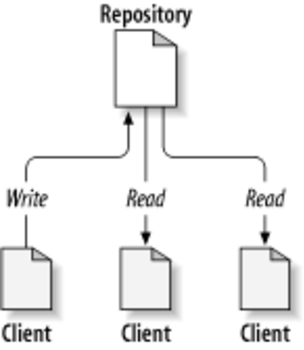
\includegraphics[width=\textwidth]{image/ch02dia1.pdf}
    \end{column}
  \end{columns}
\end{frame}

\begin{frame}[t,fragile]{URI (Uniform Resource Indicator)}
  \begin{itemize}
    \setlength{\itemsep}{1em}
  \item URI: (ネット上の)場所や名前を表す書式
    \begin{itemize}
    \item 例: URL (Uniform Resource Locator)

      {\footnotesize \url{https://wistaria@itc-lms.ecc.u-tokyo.ac.jp/lms/course/view.php?id=74564}}
    \item {\color{red}\tt https:} スキーム(scheme): プロトコル・アクセス方法を指定
    \item {\color{red}\tt wistaria@} ユーザ情報: ユーザ名(やパスワード)を指定
    \item {\color{red}\tt itc-lms.ecc.u-tokyo.ac.jp} ホスト名・サーバ名
    \item ``{\color{red}\tt //}''\ からホスト名までをオーソリティ(authority)と呼ぶ
    \item {\color{red}\tt /lms/course/view.php} パス名
    \item {\color{red}\tt ?iid=74564} クエリ(query): サーバへの指示や命令
  \end{itemize}
  \item SubversionのリポジトリのURIの例

    {\scriptsize \tt {\color{red} svn+ssh:}//{\color{blue} ce05151598@}cmp.phys.s.u-tokyo.ac.jp/home/ce05151598/svnroot}
  \end{itemize}
\end{frame}

\begin{frame}[t,fragile]{注意事項}
  \begin{itemize}
    %\setlength{\itemsep}{1em}
  \item 大きなバイナリファイル(pdf, exe, doc, tar.gz, zipなど)はなるべくsubversionで管理しない
    \begin{itemize}
      \item バイナリファイルはうまく差分が扱えない (マージできない)
    \end{itemize}
  \item チェックアウトしたディレクトリ「以外」でのファイルの編集は危い
    \begin{itemize}
      \item チェックアウト ⇒ ファイルをコピー ⇒ コピーしたファイルを変更 ⇒ チェックアウトしたディレクトリで svn update ⇒ 変更したファイルをチェックアウトしたディレクトリに戻す ⇒ svn commit ⇒ {\color{red}他の人の変更点を取り消してしまう!}
    \end{itemize}
  \item チェックアウトしたディレクトリには、管理用ディレクトリ'.svn'ができている
    \begin{itemize}
      \item チェックアウトしたオリジナルバージョンが保存されている
    \end{itemize}
  \item svn stat, svn diff はネットワークにつながってなくても使用可
  \end{itemize}
\end{frame}

\begin{frame}
  \frametitle{バージョン管理システムの欠点(面倒な点)}
  \begin{itemize}
  \item 修正前に最新の状態にアップデートしなければならない \\
   ⇒ 慣れると習慣になります
  \item 全ての修正を「コミット」しなければならない \\
    ⇒ 慣れると習慣になります
  \item 衝突(コンフリクト)が発生した時に対処しなければならない \\
    ⇒ 衝突に気づかずに修正してしまうほうが怖いです
  \item サーバのセットアップが面倒くさい \\
    ⇒ まずはホスティングサービス(github, sourceforge, bitbucket)を試してみましょう \\
    ⇒ まわりにいるプロ(?)に相談しましょう \\[.5em]
  \item バージョン管理システムを使うと作業効率が倍以上になる \\
    ⇒ {\color{red} 使わないと人生を半分損する}
  \end{itemize}
\end{frame}

\begin{frame}[t,fragile]{実習: Subversion (1)}
  \begin{itemize}
    %\setlength{\itemsep}{1em}
  \item 「ハンドブック 付録A バージョン管理システム」を読みながら以下の実習を行う
  \item リポジトリの作成 (photonにログインして作業)

    {\tt \$ \underline{svnadmin create \$HOME/svnroot}}
  \item リポジトリ内にフォルダを作成(iMacにもどって作業)

    {\tt \$~\underline{svn mkdir -m 'New folder' svn+ssh://.../svnroot/prog}}
  \item リポジトリの中をのぞいてみる

    {\tt \$ \underline{svn ls svn+ssh://.../svnroot}}

  \item リポジトリからのチェックアウト

    {\tt \$ cd \$HOME}
    
    {\tt \$ \underline{svn co svn+ssh://.../svnroot/prog}}

    ローカルに{\tt prog}ディレクトリが作成される(まだ中身は空)
  \end{itemize}
\end{frame}

\begin{frame}[t,fragile]{実習: Subversion (2)}
  \begin{itemize}
    %\setlength{\itemsep}{1em}
  \item ファイルの作成

    {\tt \$ \underline{cd prog}}
    
    {\tt \$ \underline{emacs main.c}}
  \item ファイルをsubverionの管理下に置く

    {\tt \$ \underline{svn add main.c}}
  \item 状態の確認

    {\tt \$ \underline{svn stat}}
  \item ファイルのコミット(サーバへの送信)

    {\tt \$ \underline{svn ci -m 'First version'}}
  \end{itemize}
\end{frame}

\begin{frame}[t,fragile]{実習: Subversion (3)}
  \begin{itemize}
    %\setlength{\itemsep}{1em}
  \item もう一つ別のディレクトリにチェックアウトしてみる

    {\tt \$ \underline{cd \$HOME}}
    
    {\tt \$ \underline{svn co svn+ssh://.../svnroot/prog other}}

    {\tt \$ \underline{cd other}}
    
  \item {\tt other}の下のファイルを修正、状態確認、コミット

    {\tt \$ \underline{emacs main.c}}

    {\tt \$ \underline{svn stat}}

    {\tt \$ \underline{svn ci -m 'Fixed a bug'}}
  \item {\tt \$HOME/prog}の下のファイルはそのまま
  \item 最新の状態にアップデート

    {\tt \$ \underline{cd \$HOME/prog}}

    {\tt \$ \underline{svn udpate}}
  \end{itemize}
\end{frame}

\begin{frame}[t,fragile]{実習: Subversion (4)}
  \begin{itemize}
    %\setlength{\itemsep}{1em}
  \item コミットしようとしたファイルがすでに他の人(or 他の場所)から更新されていたら
    \begin{itemize}
      \item {\color{red} コミットは失敗する}
    \end{itemize}
  \item 対処法
    \begin{itemize}
      \item まずは{\tt svn update}
      \item ファイル内の別の場所が更新されている場合: マージが成功するので、その後{\tt svn ci}
      \item ファイル内の同じ場所が更新されている場合: 衝突(コンフリクト)!

        ディレクトリ内に {\tt main.c.rXXX}, {\tt main.c.rYYY}, {\tt main.c.mine} ができる

        3つのファイルを参照しながら{\tt main.c}を編集し, {\tt svn resolved main.c}を実行した後、コミット
    \end{itemize}
  \end{itemize}
\end{frame}

\begin{frame}[t,fragile]{実習: Subversion (5)}
  \begin{itemize}
    \setlength{\itemsep}{1em}
  \item その他のコマンド
    \begin{itemize}
      \item svn mkdir dir
      \item svn move file1 file2
      \item svn copy file1 file2
      \item svn delete file
    \end{itemize}
  \item 変更履歴などを見る
    \begin{itemize}
      \item svn diff -r XXX {\ \# リビジョンXXXと現在の作業ファイル}
      \item svn diff -r XXX:YYY {\ \# 二つのリビジョン間}
      \item svn diff -c XXX {\ \# リビジョンXXX-1とXXX}
      \item svn log file
      \item svn annotate file {\ \# それぞれの行を誰がいつ変更したか}
    \end{itemize}
  \end{itemize}
\end{frame}
